\documentclass{beamer}
\usepackage{minted}


% Choose a theme (you can change this as you like)
\usetheme{CambridgeUS}

% Metadata
\title{Very SIMPLE ADD/SUB Processor}
\subtitle{Demo Simulation Report}
\author{Shein Htike}
\institute{CSC 342, Spring 2025}
\date{March 12th, 2025}

\begin{document}

% Title slide
\begin{frame}
  \titlepage
\end{frame}

% First content slide with placeholder information
\begin{frame}{Project Overview}
  \begin{itemize}
    \item \textbf{Project Title:} Very SIMPLE ADD/SUB Processor
    \item \textbf{Course:} CSC 342, Spring 2025
    \item \textbf{Instructor:} Professor Izidor Gertner
    \item \textbf{Goal:} Designing and simulating a simple processor which can execute 32-bit MIPS R-type add/subtract instructions.
    \item \textbf{Components Used:}
      \begin{itemize}
      \item 3 Port Register File (register\_file\_3port.vhd)
      \item Full Adder (full\_adder.vhd)
      \item N-bit Adder (adder\_nbit.vhd)
      \item Adder/Subtracter (adder\_subtracter.vhd)
      \item Add/Sub Processor (add\_sub\_processor.vhd)
      \end{itemize}
  \end{itemize}
\end{frame}
\begin{frame}{Instruction Format}
    The instruction format is summarized in this image below.
\begin{figure}[ht]
  \centering
  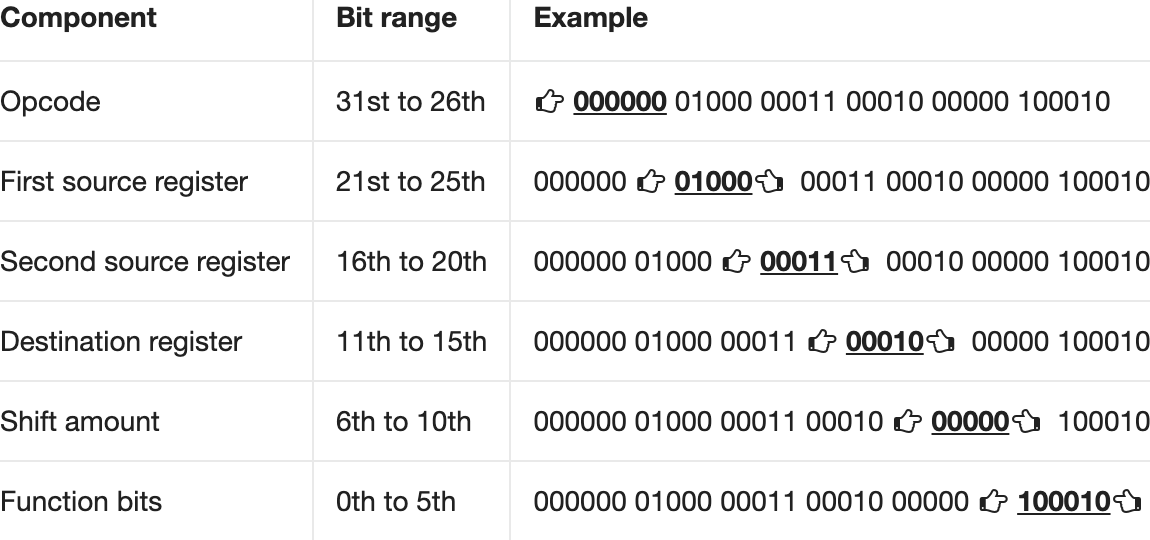
\includegraphics[width=0.8\textwidth]{./images/instructions.png}
  \caption{Instruction Format Diagram}
\end{figure}
\end{frame}
\begin{frame}{Instruction Format Cont.}
    In our case, we had four opcodes to implement.
\begin{itemize}
  \item \textbf{add (100000):} Adds two operands.
  \item \textbf{sub (100010):} Subtracts the second operand from the first.
  \item \textbf{addu (100001):} Performs unsigned addition, ignoring overflow.
  \item \textbf{subu (100011):} Performs unsigned subtraction, ignoring overflow.
\end{itemize}
Observations:
\begin{itemize}
    \item The fifth bit determines if we are adding (0) or subtracting (1).
    \item The sixth bit determines if we are detecting overflow (0) or ignoring it (1).
\end{itemize}
This will be useful when we implement these instructions.
\end{frame}
\begin{frame}[containsverbatim]{Component 1: 3 Port Register File}
    The code for the three-port register was taken from a laboratory assignment.
    It is essentially a flip-flop array with one decoder and two multiplexers. The design we were given had 8 registers, but I modified it to have 32 registers instead.
    \begin{figure}[ht]
        \centering
        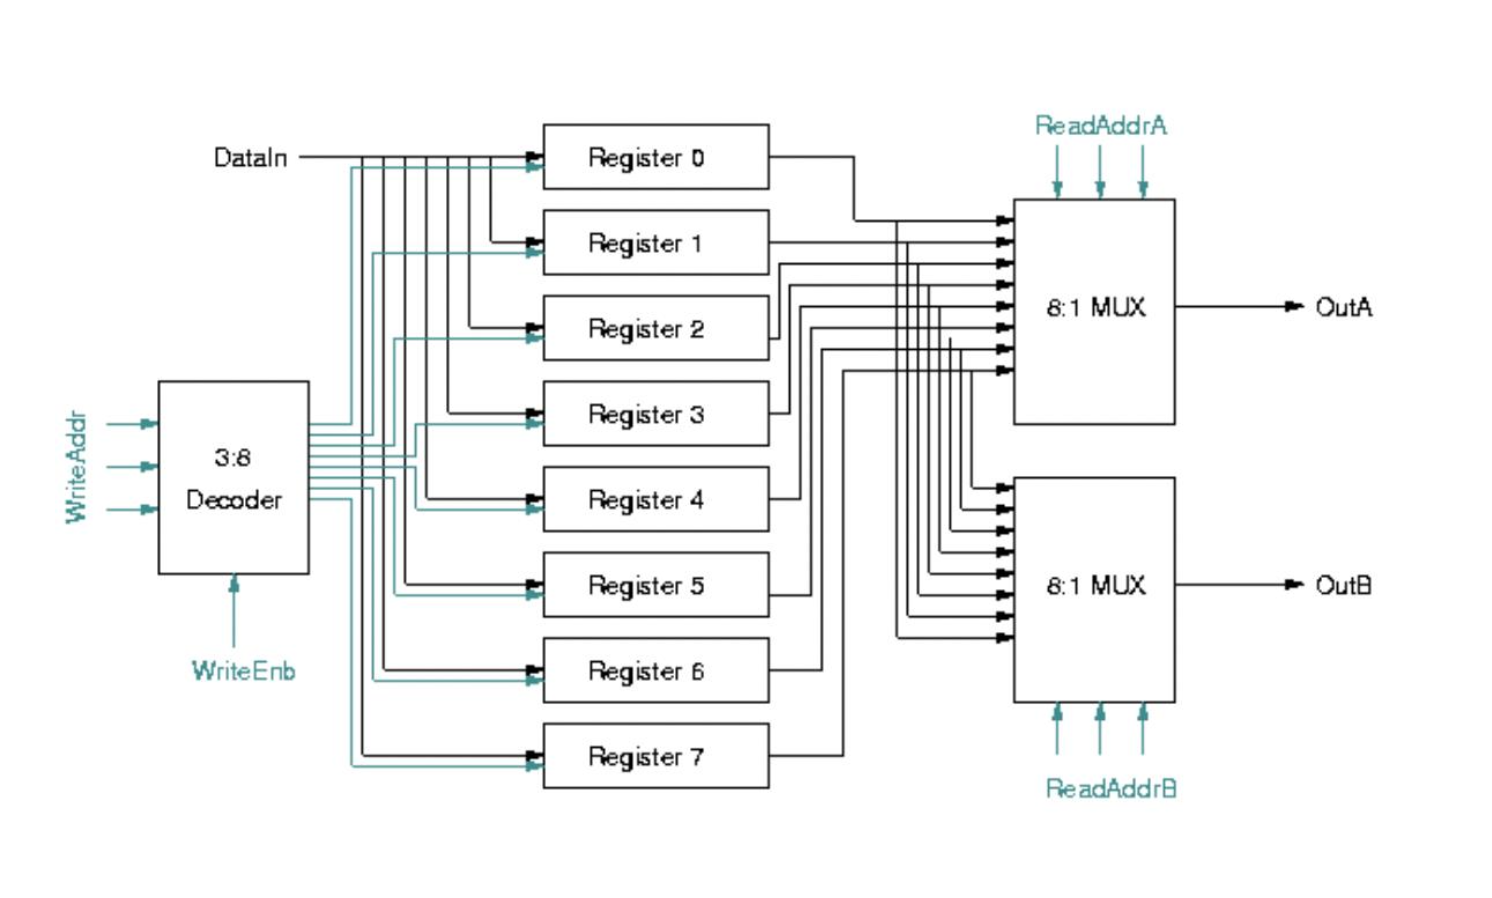
\includegraphics[width=0.8\textwidth]{./images/register.png}
        \caption{3 Port Register}
      \end{figure}
\end{frame}
\begin{frame}[containsverbatim]{Component 2: Full Adder}
    The code for the full adder was given to us in the laboratory class.
    \begin{columns}[T,onlytextwidth]
      \begin{column}{0.4\textwidth}
        {\scriptsize
        \begin{minted}{vhdl}

ENTITY full_adder IS
    PORT (
        A : IN STD_LOGIC;
        B : IN STD_LOGIC;
        CarryIn : IN STD_LOGIC;
        Sum : OUT STD_LOGIC;
        CarryOut : OUT STD_LOGIC);
END full_adder;
ARCHITECTURE dataflow OF full_adder IS
BEGIN
    Sum <= A XOR B XOR CarryIn;
    CarryOut <= (A AND B) OR ((A XOR B) AND CarryIn);
END dataflow;
        \end{minted}
        }
      \end{column}
      \begin{column}{0.6\textwidth}
        \centering
        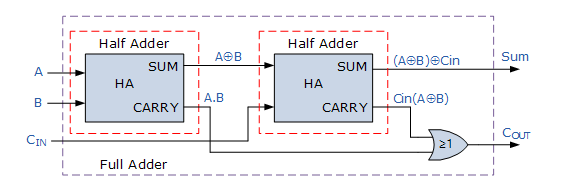
\includegraphics[width=\textwidth]{./images/full_adder.png}
      \end{column}
    \end{columns}
\end{frame}
\begin{frame}{Component 3: N-Bit Adder}
    In order to create an N-bit adder, I had to create an array of N full adders.\\
    For each adder, a signal was needed to contain the carry out signal. \\
    This carry out signal is connected to the carry in of the next adder in the line. \\
    The carry out signal of the final adder is connected to the N-bit adder's carry out. \\
    \begin{figure}[ht]
  \centering
  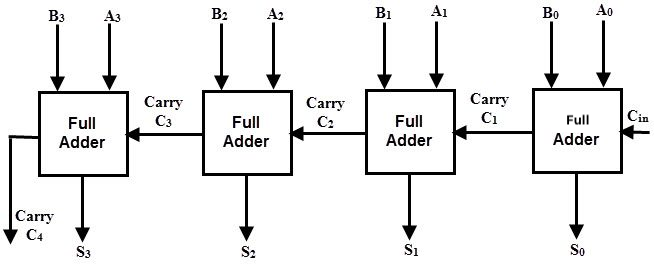
\includegraphics[width=0.5\textwidth]{./images/adder_4bit.png}
  \caption{Example of a 4 Bit Adder}
\end{figure}
\end{frame}
\begin{frame}{Component 4: Adder Subtracter}
\begin{figure}[ht]
  \centering
  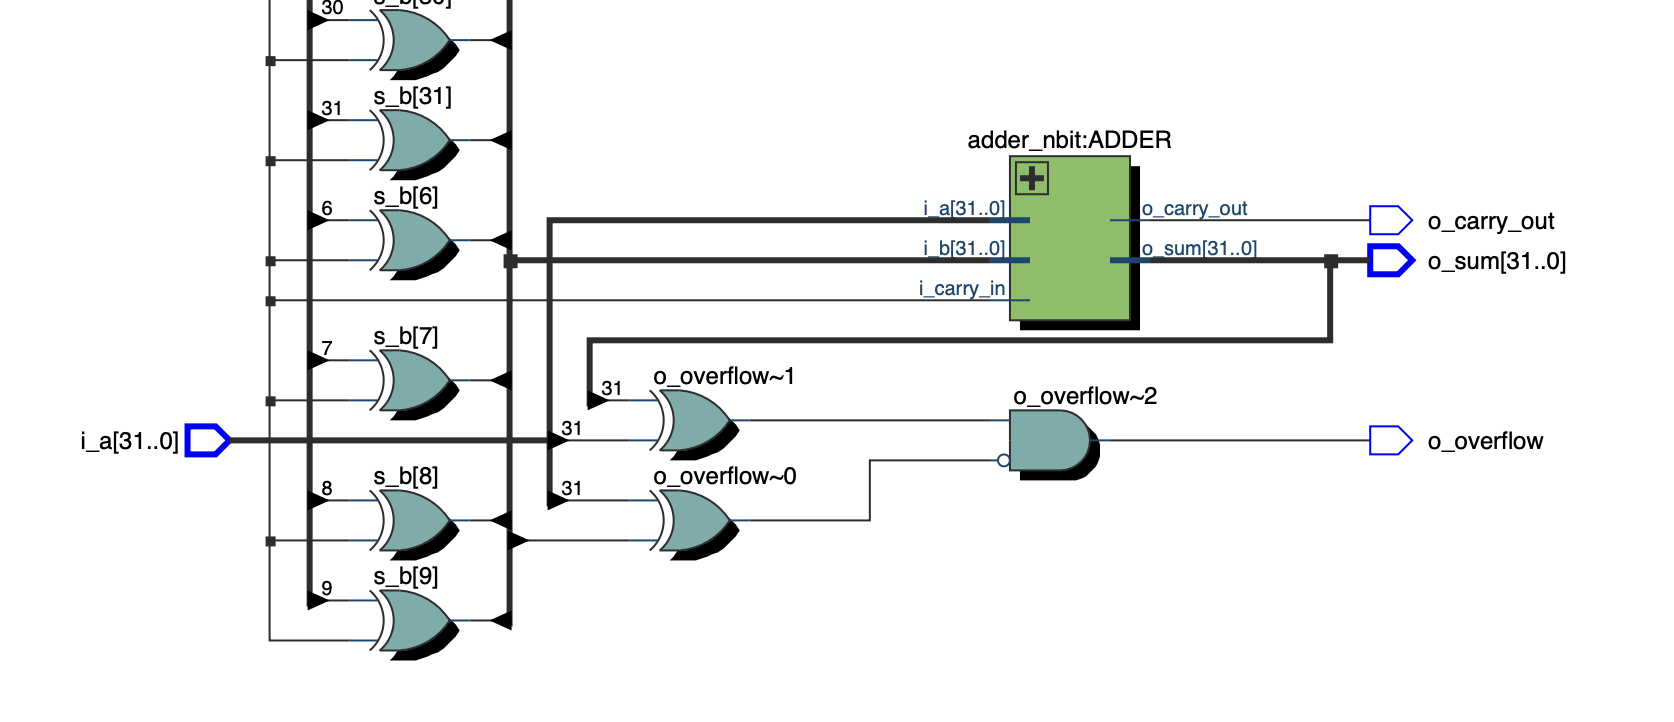
\includegraphics[width=\textwidth]{./images/adder_subtracter.png}
  \caption{Adder Subtracter Component}
\end{figure}
\end{frame}
\begin{frame}{Component 4: Adder Subtracter}
    \textbf{Subtraction Logic} \\
    We learned in class that an n-bit adder can be used as a subtractor if we flip the bits of the second operand and set carry in to 1. \\
To do this, I took the bits of the second operand and XOR'ed them with the subtraction signal. This causes the bits of the second operand to flip whenever the subtraction signal is 1. I also connected the subtraction signal into the carry-in input of my n-bit adder.
\begin{align*}
\mathtt{adder\_b} &= \mathtt{input\_b} \oplus \mathtt{add\_sub}, \\
\mathtt{adder\_cin} &= \mathtt{add\_sub}
\end{align*}
\end{frame}
\begin{frame}{Component 4: Adder Subtracter}
    \textbf{Subtraction Logic} \\
    For the ADD and SUB instructions, there needs to be overflow detection.\\
    I detected overflows by comparing the signs of the inputs to the outputs.
    \begin{align*}
    \mathtt{overflow} = (\mathtt{sign\_a} \odot \mathtt{sign\_b}) \land (\mathtt{sign\_a} \oplus \mathtt{sign\_output})
    \end{align*} 
    An overflow occurs when the sign bits of A and B match, and the sign of the output does not match the signs of A and B.
\end{frame}
\begin{frame}{Component 5: Add Sub Processor}
    \begin{figure}[ht]
        \centering
        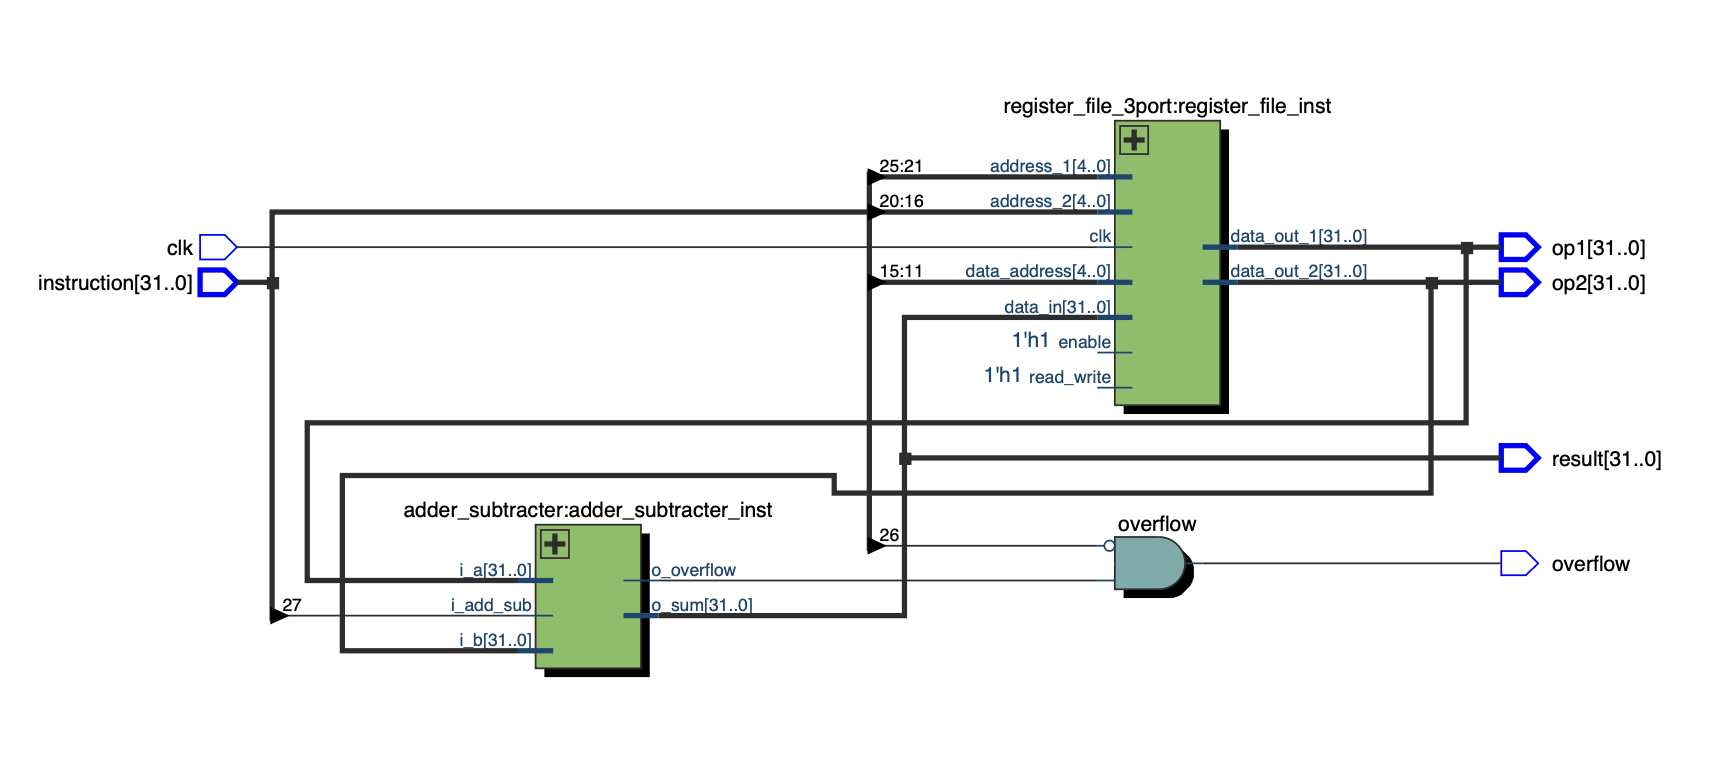
\includegraphics[width=\textwidth]{./images/add_sub_processor.png}
        \caption{Add Sub Processor}
      \end{figure}
\end{frame}
\begin{frame}{Component 5: Add Sub Processor}
    This component divides instruction and connects its bits to our components. \(shamt\) and \(funct\) are ignored.
\begin{figure}[ht]
    \centering
    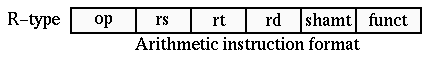
\includegraphics[width=0.7\textwidth]{./images/r_type.png}
\end{figure}

\begin{itemize}
    \item \textbf{Opcode}:
    \begin{itemize}
        \item The 5th bit is connected to \texttt{i\_add\_sub} on the adder subtracter unit.
        \item The 6th bit gets XOR'ed with our overflow output from the adder subtracter and the result is connected to the overflow signal of this component.
    \end{itemize}
    \item \textbf{Operands}:
    \begin{itemize}
        \item \texttt{rs}: Connected to address\_1 of our register file.
        \item \texttt{rt}: Connected to address\_2 of our register file.
        \item \texttt{rd}: Connected to data\_address of our register file.
    \end{itemize}
\end{itemize}
\end{frame}
\begin{frame}{Conclusion}
    This project was very interesting and gave me an understanding of how processors really work. \\
    I realized that the processors powering our devices are really nothing more than collections of logic gates such as adders and flip flops, like the components we designed.\\

    All code for this project will be available at: https://github.com/SheinH/CSC342-Add-Sub-Processor
\end{frame}
\end{document}